\chapter{总结与展望}

\section{本文工作总结}
本文围绕“包围几何上的高质量映射”展开研究。全文的组织方式可以概括为：先研究包围几何能够被稳定用作计算域所需的鲁棒内外判断，再分别围绕壳结构与高阶笼结构，构造满足不同质量目标的映射与坐标体系。对应到具体内容，本文包含一个基础问题和三项主要方法：二维曲边包围边界上的鲁棒内外判断、壳空间中的光滑双射投影、高阶笼上的闭式解析坐标，以及高阶笼上的双调和坐标。相关结果共同服务于几何属性传递、曲边笼编辑和曲线查询等任务。

本文首先研究了由有理参数曲线构成的二维包围边界上的内外判断问题。针对射线法、离散近似和局部线性化方法在复杂曲边、非严格闭合边界与脏几何场景下鲁棒性不足的问题，本文以广义环绕数为统一判据，将有理参数曲线上的相关计算转化为可闭式求解的有理积分，并进一步讨论边界点情形与导数计算。该结果为包围几何作为控制域边界、积分边界和区域组织工具提供了稳定的几何谓词基础，也为后续闭式积分推导与曲线查询任务提供了统一的计算框架。

围绕壳结构中的属性传递与对应建立需求，本文提出了高阶壳上的光滑双射投影方法。该方法从有效的线性壳出发，通过边塌缩、几何优化、边翻转和棱柱缩放等局部操作，逐步构造满足包围约束、角度约束和厚度约束的高阶壳，并在壳内构造连续向量场以定义投影算子。实验结果表明，高阶壳不仅能够在大规模模型上稳定生成，而且相较线性壳具有更光滑的投影与更均匀的壳空间分布，更适合支撑重网格化后的属性回传、布尔运算和位移贴图等应用。

围绕高阶笼中的光滑传播与角度保持需求，本文建立了 Cauchy--Green 坐标及其导数的统一闭式解析框架。与依赖中间线性笼或数值逆映射的做法不同，本文直接针对高阶输入笼推导有理积分的闭式表达，使高阶笼在保持保角形变优势的同时具备更强的边界贴合能力和更自然的交互控制方式。基于同一留数计算框架，本文进一步将相关结果扩展到 B\'{e}zier 曲线的广义环绕数查询，实现了曲边笼编辑与曲线查询之间的统一解析处理。

针对仅依赖共形坐标难以同时兼顾严格边界控制与内部低扭曲的问题，本文提出了面向高阶笼的半解析半数值双调和坐标高阶 BEM 框架。该方法通过高阶边界单元、高阶形函数和统一代数系统，将曲边边界上的双调和边值问题转化为可计算的边界元求解过程，并通过不同边界导数设计与加权策略，在严格边界插值、内部低扭曲和形变自然性之间提供连续可调的平衡机制。实验结果表明，该方法能够在复杂曲边笼编辑中得到更稳定、更自然的内部形变传播。

总体来看，本文围绕包围几何建立了从鲁棒区域判定到壳空间光滑双射投影，再到高阶笼闭式解析坐标和高阶 BEM 双调和坐标的完整方法链路。上述结果从几何构造、解析计算和数值求解三个层面推进了包围几何中的高质量映射研究，并为属性传递、交互编辑与曲线查询提供了新的理论与算法支撑。

\section{未来工作展望}
尽管本文围绕包围几何上的高质量映射建立了较完整的方法链路，但从解析求值、几何构造到交互控制，仍有若干问题值得继续深入。结合本文四项主要工作的现有局限，后续研究可重点沿以下几个方向展开。

（1）解析查询与闭式积分的鲁棒求值。
本文关于有理参数曲线广义环绕数和高阶笼闭式坐标的计算，都依赖多项式或有理方程求根、留数评估以及边界邻域处理。对于四次以上曲线，求根过程会显著影响闭式表达的计算速度与数值精度；当查询点逼近边界、出现近重根，或根的虚部接近零时，误差还可能被进一步放大。类似地，高阶壳中的沿向量投影在实现层面也会累积来自三次方程求解和重心坐标计算的数值偏差。后续可围绕高次数情形设计更稳定的求根与误差控制机制(如图~\ref{fig:chap6-quintic-rootfinding})，并系统研究边界点、近边界点和退化情形下的鲁棒求值流程，从而提升曲线查询、坐标评估和投影计算的一致性与可靠性。

\begin{figure}[htbp]
  \centering
  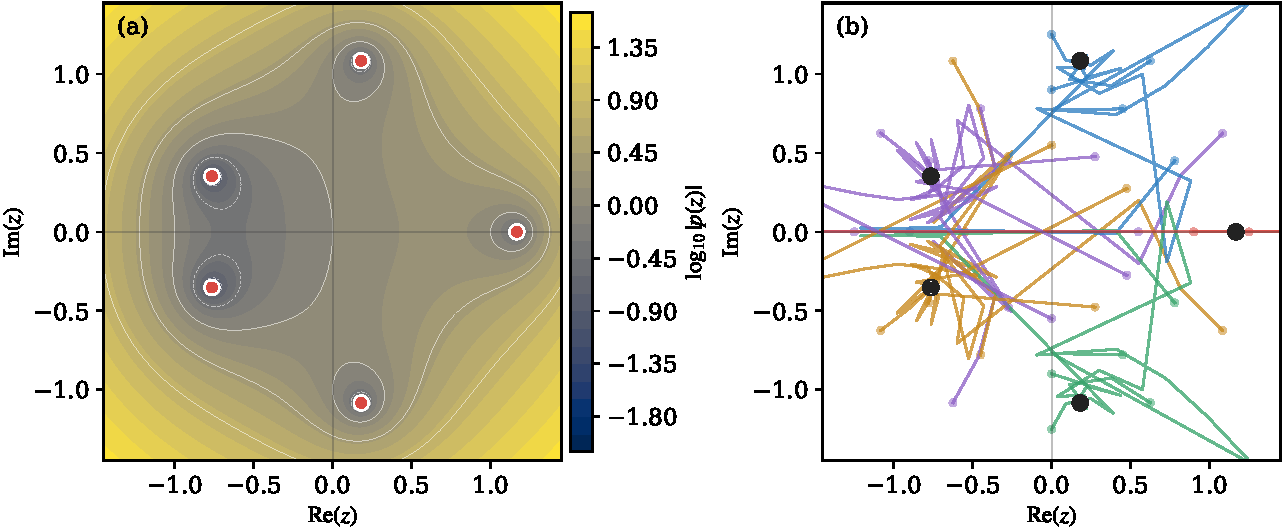
\includegraphics[width=0.9\linewidth]{figures/chap6_quintic_rootfinding.pdf}
  \caption{五次多项式求根示意。这里以 \(p(z)=z^5-z-1\) 为例，左图给出复平面上的 \(\log_{10}|p(z)|\) 分布，右图给出若干初值在 Newton 迭代下收敛到五个根的轨迹。}
  \label{fig:chap6-quintic-rootfinding}
\end{figure}

（2）从二维高阶边界到三维高阶边界的推广。
目前本文关于广义环绕数、Cauchy 坐标和双调和坐标的核心结果主要建立在二维高阶笼与二维参数曲线上，而三维模型与三维包围结构在图形学和工程建模中更为常见。因此，将现有方法推广到三维高阶笼、曲面笼以及三维参数曲面，是后续最自然也最具挑战性的方向之一。图~\ref{fig:chap6-3dwind} 所示的三维环绕数问题与图~\ref{fig:chap6-3dcage} 所示的 cage 形变结果，正对应了三维场景下区域判定与边界控制这两类典型需求。对于广义环绕数而言，需要面对三维参数曲面上更复杂的积分结构与奇异性分析；对于 Cauchy 坐标和双调和坐标而言，则需要重新处理三维边值问题、边界表示和导数控制之间的关系。特别是双调和坐标虽然理论上可以延伸到三维，但其高阶边界元构造与解析表达都会明显更复杂，这意味着需要新的解析工具与数值离散策略。

\begin{figure}[htbp]
  \centering
  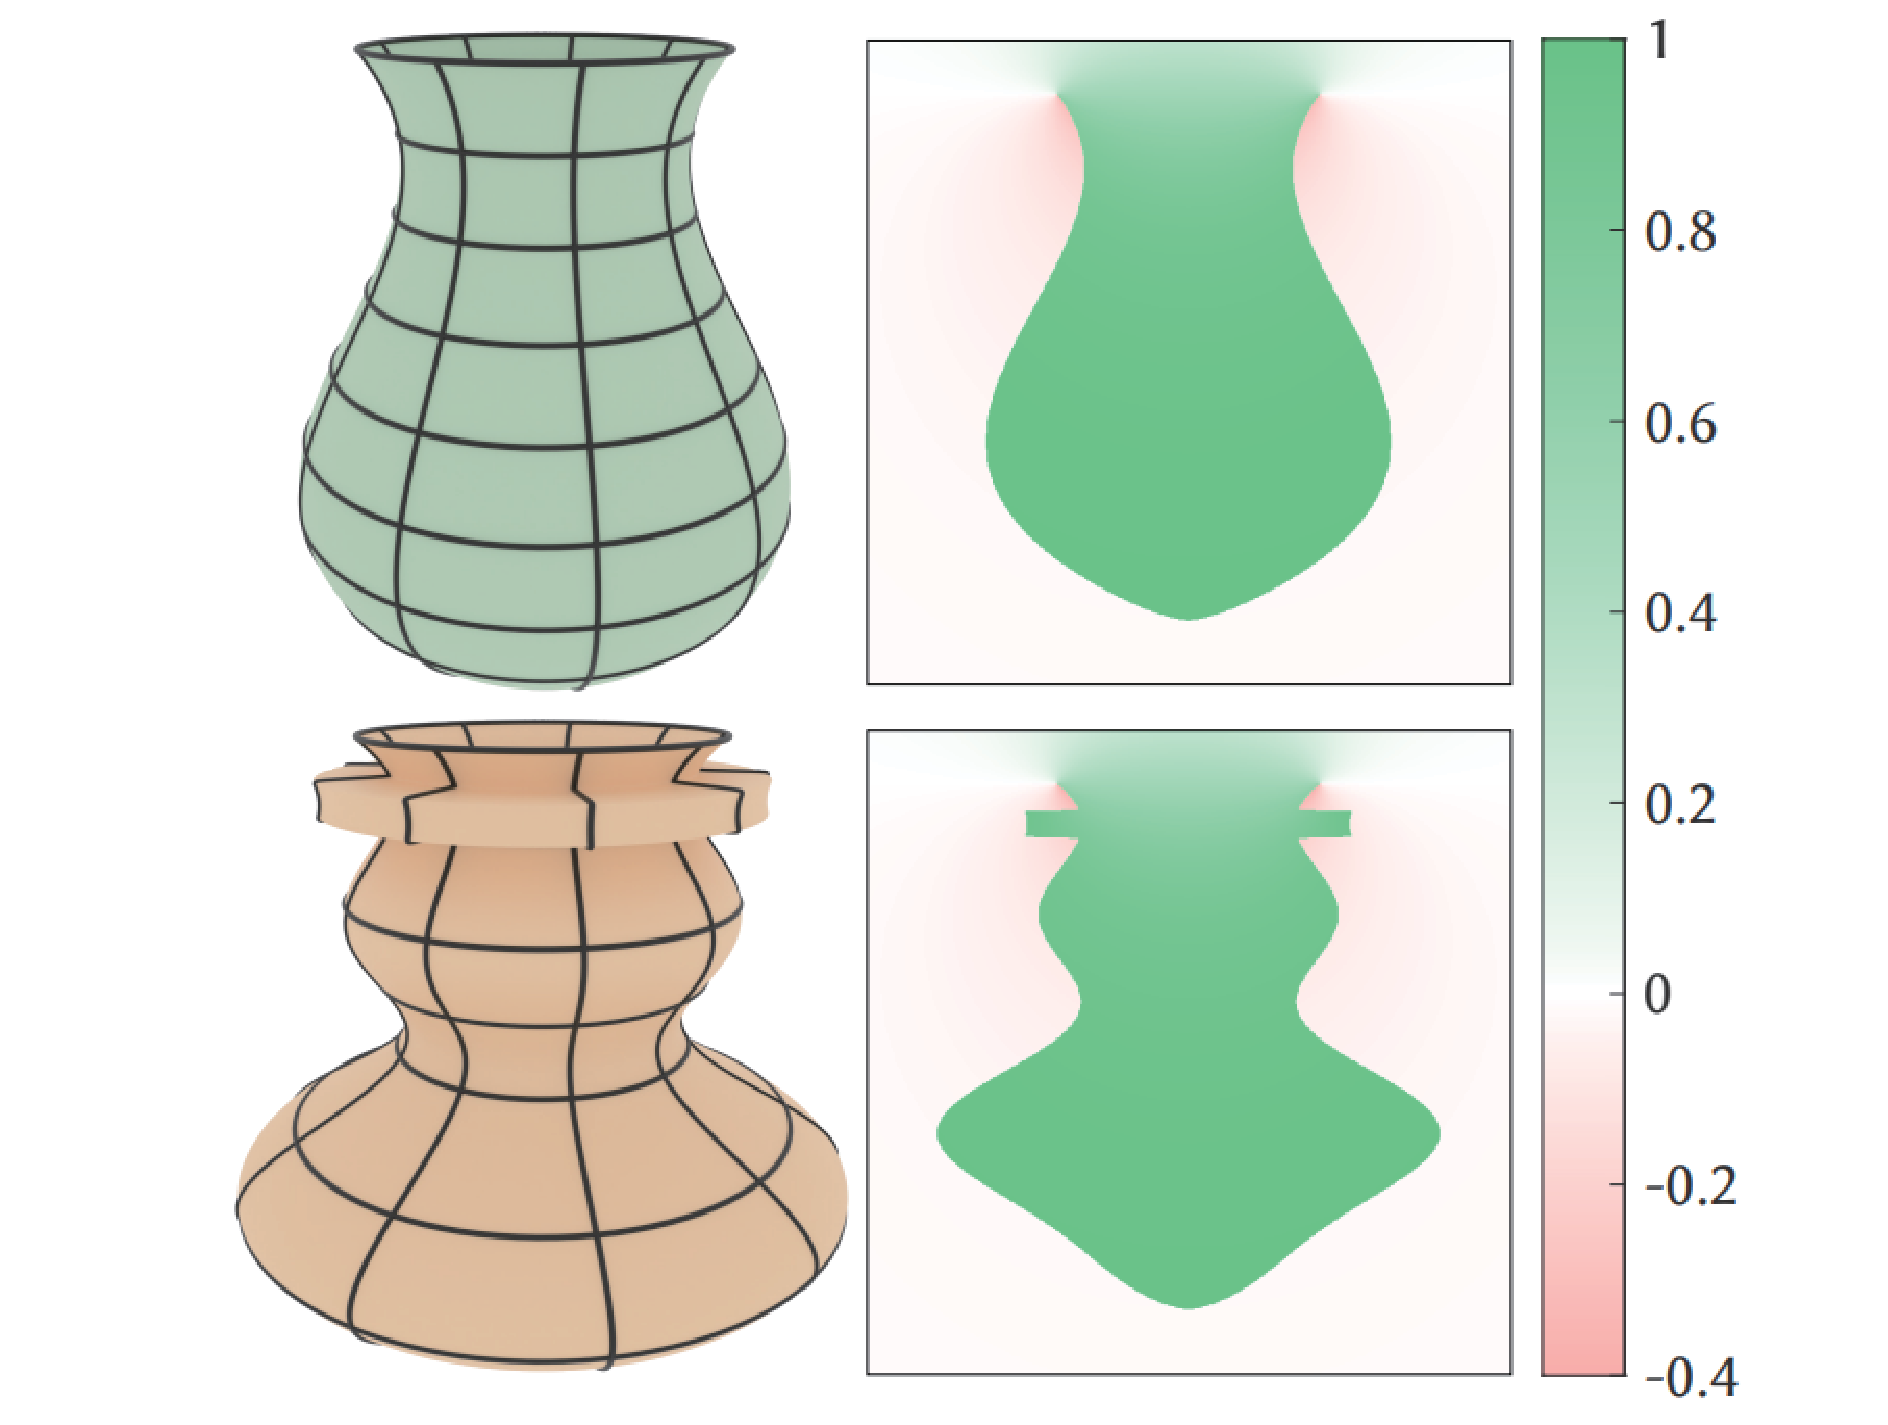
\includegraphics[width=0.82\linewidth]{figures/chap7_3Dwind.pdf}
  \caption{三维情形下对应的环绕数。}
  \label{fig:chap6-3dwind}
\end{figure}

\begin{figure}[htbp]
  \centering
  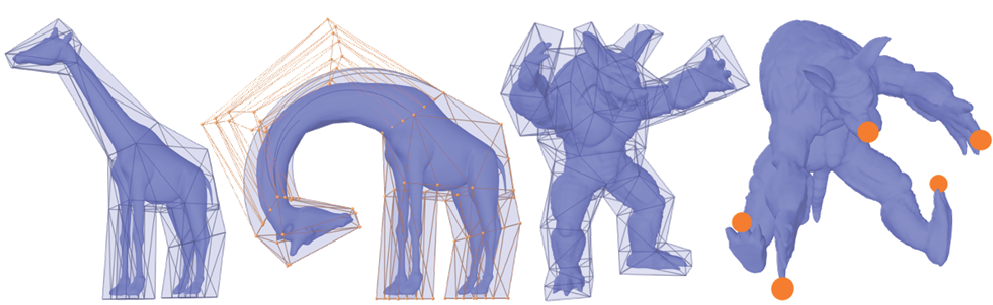
\includegraphics[width=0.99\linewidth]{figures/chap7_3Dcage.pdf}
  \caption{三维情形下的 cage 对应形变结果。}
  \label{fig:chap6-3dcage}
\end{figure}

（3）更易用的高阶笼编辑机制。
高阶笼能够以更少的几何单元贴合复杂边界，但当前方法仍要求用户显式给定较多的变形曲线，或直接调整较多控制点。在实际编辑中，这种控制方式虽然表达能力强，却也提高了交互门槛。另一方面，共形性与严格插值之间本身存在冲突，因此形变结果未必始终紧密跟随编辑后的笼边界，这会进一步增加用户调整结果的难度。后续可考虑在高阶笼框架中引入变分式控制方式，用更少的高层控制量驱动整体变形；同时研究允许用户在局部区域放松共形约束、区分不同区域形变优先级的机制，从而在边界跟随性、角度保持和交互直观性之间取得更灵活的平衡。

（4）壳空间构造的理论保证与复杂输入扩展。
本文的高阶壳在实验中表现出比线性壳更光滑的投影和更均匀的受限空间，但这种均匀性目前仍缺乏严格理论保证。其原因在于，壳构造过程同时受到包围约束、角度约束和厚度约束的限制，而中层 \Bezier 三角面目前主要通过较简单的拟合方式获得，再据此生成上下表面，因此在均匀厚度和壳空间分布方面仍有改进空间。后续可进一步研究更合理的中层曲面构造方式和厚度分配策略，分析壳空间均匀性、厚度变化与投影稳定性之间的关系。与此同时，现有壳方法仍主要面向流形且可定向的输入，对非流形、含边界或更一般的非刚性对应问题支持有限，也尚难将已有重网格化流程直接作为黑盒调用。这些问题若能得到解决，将显著提升壳空间方法在复杂工程模型上的适用范围。

（5）统一且高效的包围几何处理管线。
从实现角度看，当前高阶壳构造中相当一部分时间消耗在约束检查以及中、上、下 \Bezier 三角面的生成上；而闭式曲线查询和高阶笼坐标计算也各自包含一套独立的解析与数值处理流程。后续可进一步探索如何减少约束检查次数、改进 \Bezier 三角面的构造策略，并将鲁棒内外判断、壳空间投影、闭式解析坐标和高阶 BEM 双调和坐标更紧密地组织到统一框架中。这样不仅有助于减少不同模块之间的重复计算，也有利于面向重网格化、属性传递、曲边编辑和 CAD 前处理等任务，构建更加一致的包围几何处理流程。

总体而言，包围几何仍是数字几何处理中兼具理论价值与工程价值的重要中间表示。随着高阶边界表示、解析积分方法和高质量映射构造技术的进一步发展，围绕“更鲁棒的查询、更自然的编辑、更严格的理论保证以及更统一的处理流程”的研究，将持续推动包围几何在属性传递、交互设计与复杂几何处理中的应用深度与广度。
